\documentclass[12pt,a4paper,openany,oneside]{book}

%%%%%%%%%%%%%%%%%%%%%%%%
% Imports
%%%%%%%%%%%%%%%%%%%%%%%%
\usepackage{hyperref} % Extensive support for hypertext in LATEX (https://ctan.org/pkg/hyperref)
\usepackage[utf8]{inputenc}
\usepackage[italian]{babel}
\usepackage{csquotes}
\usepackage{graphicx} % Enhanced support for graphics (https://ctan.org/pkg/graphicx)
\usepackage{framed} % Framed or shaded regions that can break across pages (https://ctan.org/pkg/framed)
\usepackage[toc,acronyms]{glossaries}
\usepackage[font=small,labelfont=bf,tableposition=top]{caption}
\usepackage[style=numeric,useprefix,hyperref,backend=bibtex,sorting=none]{biblatex} % Sophisticated Bibliographies in LATEX (https://ctan.org/pkg/biblatex)
\usepackage{listings}
\usepackage{subfig}

%%%%%%%%%%%%%%%%%%%%%%%%
% Settings
%%%%%%%%%%%%%%%%%%%%%%%%
\renewcommand*{\figureautorefname}{Fig.}
\renewcommand*{\sectionautorefname}{sez.} 
\renewcommand*{\chapterautorefname}{Cap.} 
\graphicspath{ {./img/} } % Base image path
\lstset{
    language=C++,
    basicstyle=\footnotesize\ttfamily,
    numbers=left,
    numberstyle=\tiny,
    numbersep=5pt,
    tabsize=5,
    extendedchars=true,
    breaklines=true,
    keywordstyle=\textbf,
    stringstyle=\color{white}\ttfamily,
    showspaces=false,
    showtabs=false,
    xleftmargin=17pt,
    framexleftmargin=17pt,
    framexrightmargin=5pt,
    framexbottommargin=4pt,
    showstringspaces=false
}

%%%%%%%%%%%%%%%%%%%%%%%%
% References
%%%%%%%%%%%%%%%%%%%%%%%%
\addbibresource{resources.bib} %Import the bibliography file

%%%%%%%%%%%%%%%%%%%%%%%%
% Glossary
%%%%%%%%%%%%%%%%%%%%%%%%
\makenoidxglossaries
\loadglsentries{glossary}

%%%%%%%%%%%%%%%%%%%%%%%%
% Begin document
%%%%%%%%%%%%%%%%%%%%%%%%
\begin{document}

% Metadata
\title{EWT summary}
\author{Ernesto Casablanca}
\date{\today}

% Title page
\begin{titlepage}
    \centering 
    
\includegraphics[width=2.434cm,height=2.565cm]{university_logo.png}

    \bigskip

    {\Large \textbf{UNIVERSIT\`A DEGLI STUDI DI CATANIA}}

    {\scshape
        \large
        Dipartimento di Matematica e Informatica
    }
    {\scshape
        \normalsize
        Corso di Laurea Triennale in Informatica
    }

    \bigskip

    \hrule

    \bigskip
    \bigskip
    \bigskip
    \bigskip

    {\itshape
        \large
        Ernesto Casablanca
        \par}

    \bigskip
    \bigskip
    \bigskip
    \bigskip

    {\centering
        \Large
        Decentralizzazione del mercato dell'energia
        \par}
    {\centering
        Decentralization of the energy market
        \par}

    \bigskip
    \bigskip
    \bigskip
    \bigskip
    \bigskip
    \bigskip

    \begin{minipage}[b]{8 cm}
        \hrule
        \bigskip
        {\centering\scshape
            Relazione Progetto Finale
            \par}
        \bigskip
        \hrule
    \end{minipage}

    \bigskip
    \bigskip
    \bigskip
    \bigskip
    \bigskip
    \bigskip
    \bigskip
    \bigskip
    \bigskip
    \bigskip
    \bigskip

    {\raggedleft
        Relatore: Prof. Giuseppe Pappalardo \\
        Correlatore: Dott. Giovanni Marotta
        \par}

    \bigskip
    \bigskip
    \bigskip
    \bigskip

    \hrule

    \bigskip

    {\centering
        Anno Accademico 2020 - 2021
        \par}

\end{titlepage}


% Index
\tableofcontents

% Abstract
\chapter*{Abstract}
\addcontentsline{toc}{chapter}{Abstract} % add the chapter to the index

%%%%%%%%%%%%
% Content
%%%%%%%%%%%%
Il mondo della produzione e distribuzione dell'energia elettrica sta andando incontro ad un processo di decentralizzazione sempre più rapido. \\
La spinta nasce dall'ingresso nel mercato di nuovi piccoli produttori di energia rinnovabile con capacità variabili e 
da una domanda che necessita di sempre più flessibilità e con una rinnovata sensibilità ambientale. \\
Per poter supportare questo nuovo tipo di mercato, incentrato su un rapporto più diretto fra produttore e consumatore, 
diversi progetti hanno preso in considerazione la tecnologia delle blockchain, sfruttandone i punti di forza e cercando di superarne le limitazioni. \\
In questo documento ci si concentrerà particolarmente sulle soluzioni in questo ambito proposte dal progetto Energy Web, 
al fine di fornire un esempio concreto di una possibile implementazione. \\
I concetti chiave possono comunque essere applicati ad altri progetti della stessa natura.

% Introduction
\chapter{Introduzione}
TODO

\begin{figure}[t] %[t] per inserire la figura in cima alla pagina
	
\includegraphics[width=1\linewidth]{university_logo.png} %width=1\linewidth per scalare l'immagine alle dimensioni opportune. E' possibile ridurre le dimensioni dell'immagine inserendo un numero minore di 1
	\caption{Questo è un esempio di didascalia.}
	\label{fig:immagine} %per poter richiamare l'immagine nel testo
\end{figure}


\begin{lstlisting}[caption={Didascalia},label=lst:multicorrelation]
double multicorrelation_ncc(template_obj,candidate_obj) {
double similarity = ncc(template_obj,candidate_obj);
if (similarity<t) {
split template_obj into blocks: template_obj[9];
split candidate_obj into blocks:  candidate_obj[9];
similarity=0;
for (i=0; i<9; i++)
similarity+=ncc(template_obj[i],candidate_obj[i]);
similarity/=9;
}
else
return similarity;
}
\end{lstlisting}

% \begin{table}[ht]
% 	\begin{center}
% 		\caption{Tabella Generica}\label{tab:gen}
% 		\begin{tabular}{lcccccc}

% 			& & & & & & \\ \hline
% 			\multicolumn{1}{|c}{}  & \multicolumn{5}{|c|}{\bf Y} &
% 			\multicolumn{1}{c|}{} \\

% 			\multicolumn{1}{|c}{\bf X} & \multicolumn{1}{|c}{$1$} & $\ldots$ & $j$ & $\ldots$ &
% 			\multicolumn{1}{c|}{$k$} & \multicolumn{1}{c|}{$\Sigma_{j=1}^k{X_{ij}}$} \\ \hline

% 			\multicolumn{1}{|c}{$1$} & \multicolumn{1}{|c}{$X_{11}$} & $\ldots$ & $X_{1j}$ &
% 			$\ldots$ & \multicolumn{1}{c|}{$X_{1k}$} &
% 			\multicolumn{1}{c|}{$m$}\\

% 			\multicolumn{1}{|c}{$\vdots$} & \multicolumn{1}{|c}{$\vdots$} &  & $\vdots$ &  &
% 			\multicolumn{1}{c|}{$\vdots$} &
% 			\multicolumn{1}{c|}{$\vdots$}\\

% 			\multicolumn{1}{|c}{$i$} & \multicolumn{1}{|c}{$X_{i1}$} & $\dots$ & $X_{ij}$ &
% 			$\ldots$ & \multicolumn{1}{c|}{$X_{ik}$} &
% 			\multicolumn{1}{c|}{$m$} \\

% 			\multicolumn{1}{|c}{$\vdots$} & \multicolumn{1}{|c}{$\vdots$} &
% 			& $\vdots$ &  & \multicolumn{1}{c|}{$\vdots$} & \multicolumn{1}{c|}{\vdots} \\

% 			\multicolumn{1}{|c}{$n$} & \multicolumn{1}{|c}{$X_{n1}$} & $\dots$ & $X_{nj}$ &
% 			$\ldots$ & \multicolumn{1}{c|}{$X_{nk}$} & \multicolumn{1}{c|}{$m$}\\ \hline

% 		\end{tabular}
% 	\end{center}
% \end{table}

% Energy web
\chapter{Energy web}

%%%%%%%%%%%%
% Content
%%%%%%%%%%%%
\section{Cos'è Energy Web}
\gls{ew} è un progetto nato nel 2017 con sede in Zugo, Svizzera \cite{wiki:ew-history}. 
Ad affiancarlo e dargli valore vi sono molti partner commerciali, comprese aziende molto conosciute nel settore energetico \cite{wiki:ew-affiliate}. \\
L'obiettivo prefissato da \gls{ew} è quello di spingere per uno sviluppo del settore che punti verso un abbassamento delle emissioni di carbonio e che sia in grado di gestire la decentralizzazione del mercato delle risorse.
Per farlo, \gls{ew} utilizza tecnologie distribuite e open-source dalle quali partire per realizzare un'infrastruttura commerciale specifica per l'ambito energetico \cite{wiki:ew-about}. \\
Nel 2019, \gls{ew} ha rilasciato \gls{ewc}, una blockchain pubblica basata su Ethereum, sulla quale si basa l'intero ecosistema di \gls{ew}: \gls{ewdos}.

\section{EW-DOS}
Il cuore del progetto di \gls{ew} è \gls{ewdos}, un'infrastruttura digitale open-source ad accesso pubblico e decentralizzato. \\
L'idea è quella di fornire un insieme di strumenti e servizi che rendano il più semplice possibile lo sviluppo di \gls{dapp} mirate al settore energetico, 
anche se, ovviamente, le varie tecnologie possono essere applicate anche ad ambiti più generici. \\
L'intero sistema è stato pensato come tre strati sovrapposti, in cui ogni strato si basa su quello sottostante per implementare ulteriori funzionalità, come mostrato in \autoref{lab:ew-dos}. \\

I tre strati sono:
\begin{itemize}
    \item Trust - \gls{ewc}
    \item Utility - Servizi e astrazioni sopra la blockchain
    \item Toolkit - Frameworks e toolkit per la costruzione di applicazioni
\end{itemize}

\begin{figure}[h]
    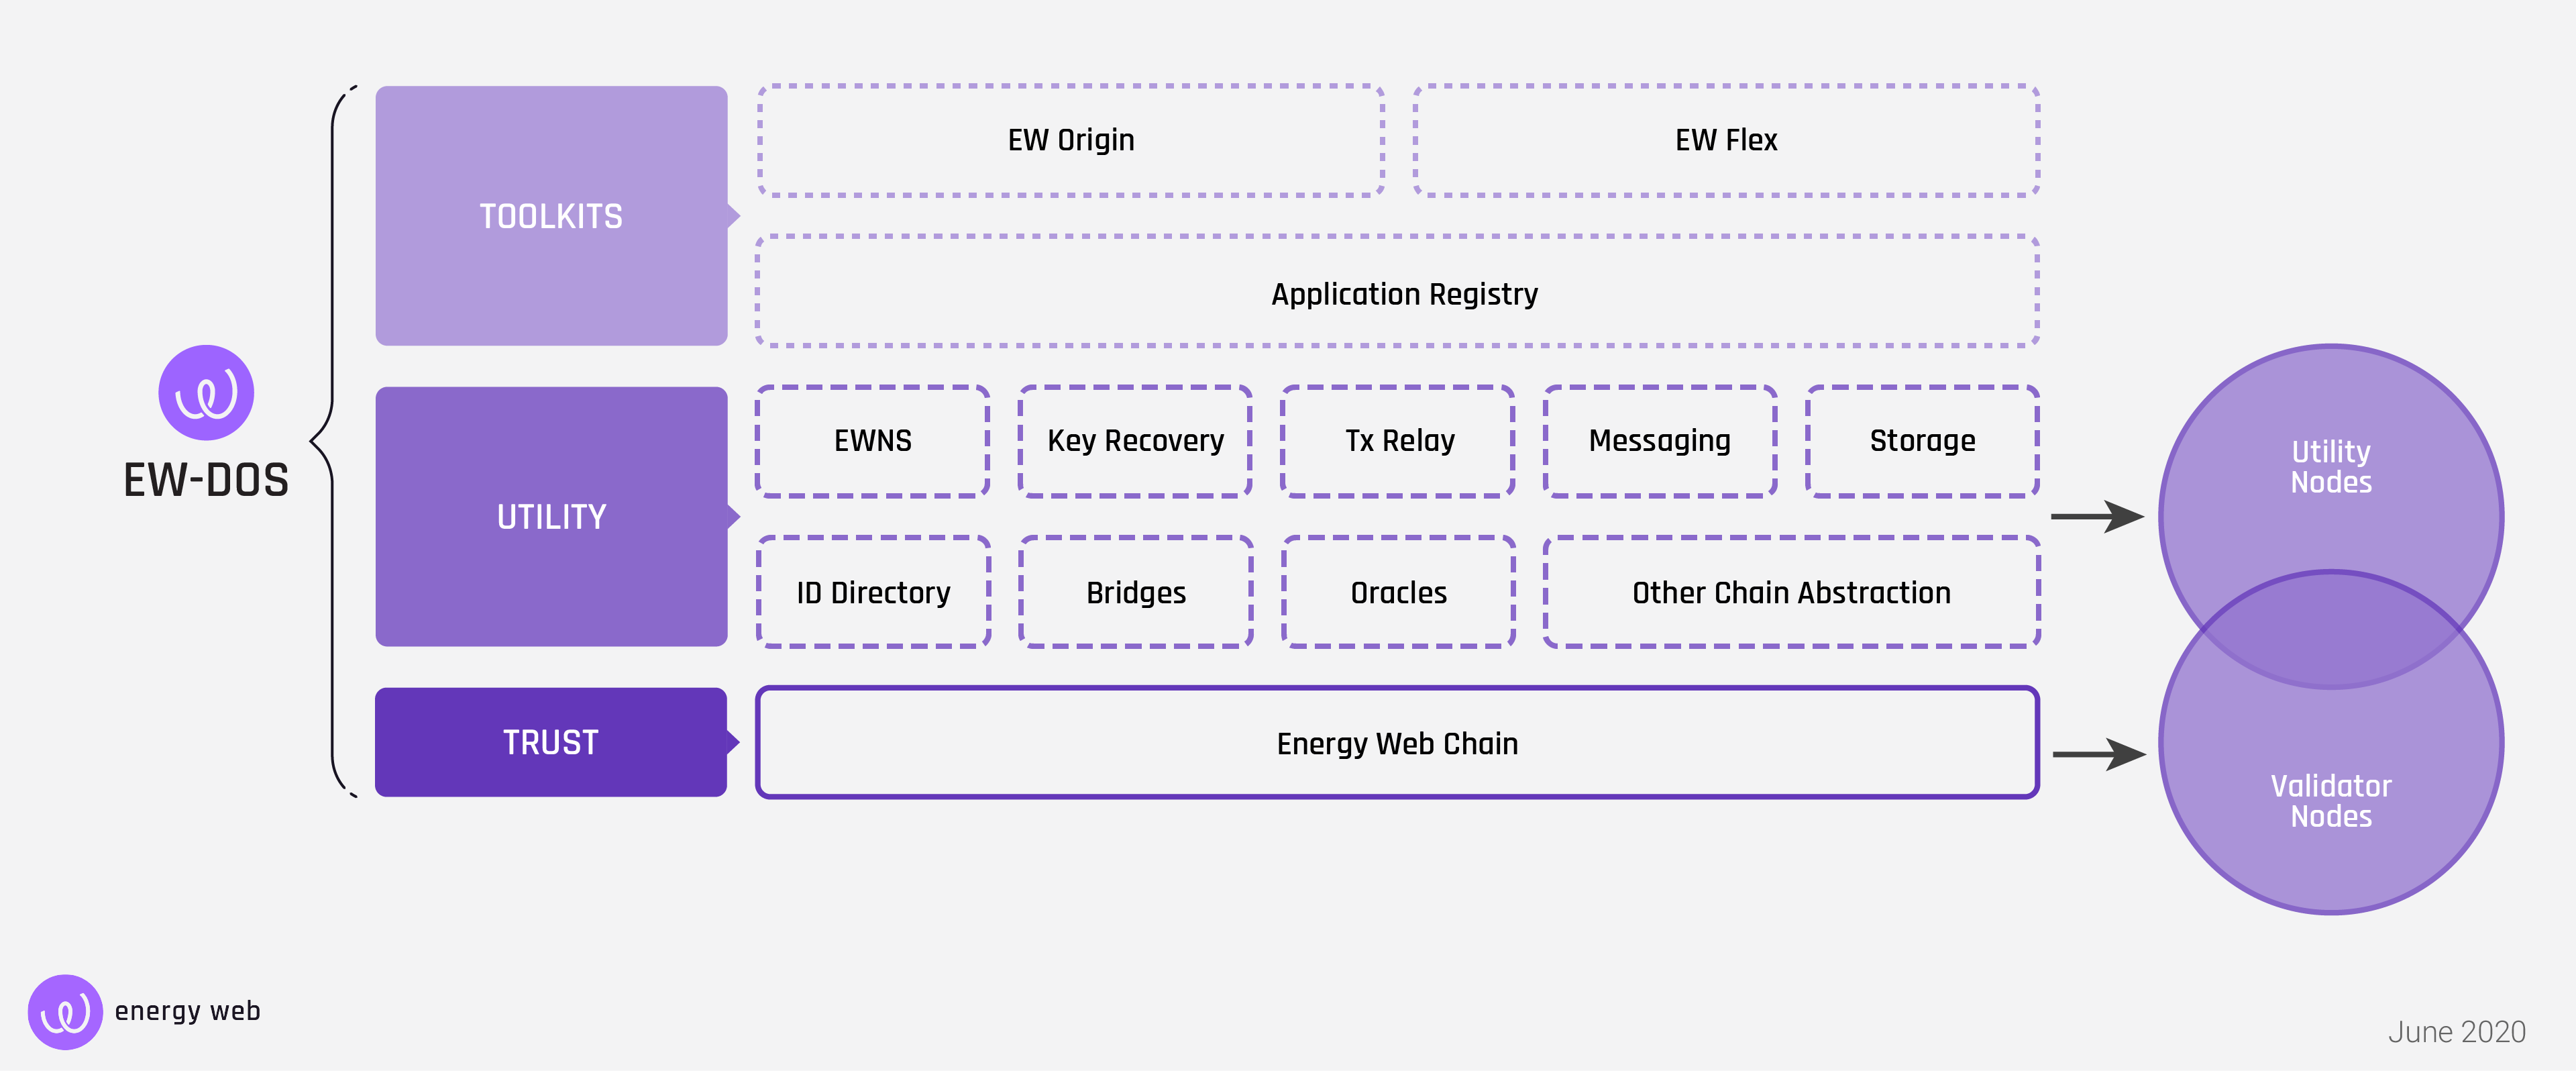
\includegraphics[width=13cm]{ew-dos}
    \centering
    \caption{Visualizzazione della struttura di \gls{ewdos} \cite{img:ew-dos}}
    \label{lab:ew-dos}
\end{figure}

\section{Trust}
Il livello Trust comprende la \gls{ewc} (cfr. \autoref{cap:ew}), 
il cui ruolo principale è quello di assicurare che ci sia consenso sui dati e che tutte le applicazioni e gli smart contracts si comportino in maniera deterministica. \\
Si tratta di una blockchain basata su Ethereum, \gls{evm} inclusa, e rispetta tutti gli \gls{erc}. \\
Il token digitale per il pagamento delle transazioni e dei servizi offerti dalla piattaforma è l'\gls{ewt} e l'algoritmo di consenso è il \gls{poa}. \\
È presente anche una test-net, chiamata Volta, usata per testare i progetti e le applicazioni prima di lanciarle sulla main-net. 

\section{Utility}
Il livello di utility è composto da un insieme di servizi basati sulla \gls{ewc} che hanno lo scopo di rendere quanto più accessibile e invitante possibile l'intera infrastruttura per gli sviluppatori di DApp,
ed inoltre mettendo a disposizione un gran numero di smart contracts per il backend e di librerie per il frontend \cite{art:ew-dos}. \\
Come anticipato, il pagamento di servizi del livello di Utility della piattaforma vengono pagati in EWT. \\
I nodi della blockchain che forniscono queste funzionalità sono chiamati Utility Nodes, e vengono ricompensati attraverso il meccanismo dello Staking (cfr. \autoref{sec:staking}).\\

È possibile individuare tre ampie categorie di servizi:
\begin{itemize}
    \item Esperienza dell'utente finale
    \item Interoperabilità Multipiattaforma
    \item Performance delle applicazioni
\end{itemize}

\subsection{Esperienza dell'utente finale}
\begin{itemize}
    \item \gls{ewns} - Similmente ad un DNS, associa domini arbitrari ad indirizzi sulla blockchain
    \item DID Key Recovery - Permette il recupero della propria DID  (cfr. \autoref{sec:did})
    nel caso si fosse persa la chiave privata
    \item Transaction Relay - Servizio che fa da intermediario fra un cliente e la blockchain, nascondendo l'utilizzo della stessa e simulando una più tradizionale interazione client-server
\end{itemize}

\subsection{Interoperabilità Multipiattaforma}
\begin{itemize}
    \item Bridges - Consente il trasferimento di token fra blockchain diverse. Attualmente è utilizzato per collegare \gls{ewc} con Ethereum
    \item Oracles - Particolari nodi che è possibile consultare con il protocollo Chainlink per ricevere dati di eventi esterni alla blockchain \cite{art:oracles} \cite{wiki:oracles} 
\end{itemize}

\subsection{Performance delle applicazioni}
\begin{itemize}
    \item Identity Directory - Smart contract che contiene tutti le \gls{did}
    \item Messaging - Un sistema di messaggistica che sfrutta le \gls{did} per assicurare validità ed autenticità dei messaggi
    \item Storage - L'utilizzo di sistemi di storage distribuiti esterni, come IPFS \cite{wiki:ipfs}  rende possibile limitare al minimo indispensabile la quantità di dati salvati sulla blockchain
\end{itemize}

\section{Toolkit}
Il livello toolkit comprende una serie di framework ed applicazioni di esempio utili per realizzare \gls{dapp} che sfruttino al massimo le funzionalità di \gls{ewdos} \cite{art:ew-dos}.
Sebbene siano pensati per il settore energetico, la loro natura open-source li rende ottime basi di partenza per costruire soluzioni anche per altri ambiti.

\subsection{Application Registry}
Architettura in grado creare registri di \gls{did} che verifichino che soddisfino la condizione specificata, come ad esempio la località geografica o il possesso di una certa qualifica.

Questo registro sarà poi utilizzato da una \gls{dapp} per creare un servizio di autorizzazione e autenticazione. 

Ogni \gls{dapp} deve fare riferimento ad un Application Registry, che può essere riutilizzato in più applicazioni.

\subsection{EW origin}
Framework per sviluppare applicazioni che supportino il tracciamento, la trasmissione e il conferimento di \gls{eac} alle \gls{res} secondo gli standard del settore. 

I due attori principali sono il Registry e l'Issuer. 
Il primo salva e amministra le informazioni legate ad utenti e \gls{der}, con la possibilità di mantenere dati potenzialmente sensibili off-chain, cioè utilizzando dello storage al di fuori della blockchain.
Il secondo potrà essere utilizzato dalle autorità competenti per coniare nuovi \gls{eac} che siano tracciabili, con una implementazione basata sullo standard ERC-1155.

\subsection{EW flex}
Software open source attualmente in sviluppo per la gestione dei \gls{der} e le operazioni che li coinvolgono, 
permettendone una facile connessione alla rete e sottoponendo le offerte ad un operatore autorizzato \cite{art:ew-dos}. \\

Sarà composto dai seguenti moduli:

\begin{itemize}
    \item Flex Nodes - Cluster di nodi che eseguono materialmente la business logic che gestisce offerta e domanda, e le accoppia secondo quanto stabilito dall'operatore responsabile.
    \item Flex Clients - Insieme di tutti i \gls{der} che partecipano al mercato dell'energia, inclusi dispositivi \gls{iot}
    \item Flex Bridge - Modulo che permette la comunicazione e la coordinazione con gli operatori della rete elettrica
    \item Flex Governance - Serie di smart contracts che governano i Flex Nodes. Permettono agli enti predisposti di imporre le regolamentazioni vigenti
\end{itemize}

% Energy web chain
\chapter{Energy Web chain}
\label{cap:ew}

%%%%%%%%%%%%
% Content
%%%%%%%%%%%%
\section{Confronto con Ethereum}
Non è un mistero che la \gls{ewc} sia basata su Ethereum, più precisamente sulla sua ottava hard-fork, Istanbul \cite{wiki:ew-fork}. 
È in programma una ulteriore migrazione alla hard-fork Berlino, che avverrà quanto prima \cite{wiki:ew-berlino}. \\
Anche alcuni dei servizi offerti, come l'\gls{ewns} sono fork con modifiche minime di progetti nati su Ethereum. \\

Tuttavia, ci sono alcuni aspetti in cui le due reti differiscono, come riassunto nella segunte tabella: \\

\hskip-.6cm
\begin{tabular}{||p{6cm}|p{7cm}||}
    \hline
    Problema                                                    & Modifica                                                                                                                    \\
    \hline\hline
    Basso throughput, alti costi, scalabilità limitata          & Utilizzo della \gls{poa}: incrementa il throughput fino a 30x                                                               \\
    \hline
    Poco adatta a piccoli dispositivi (IoT)                     & Maggiore focus sui \textbf{light client} per connettere anche piccoli dispositivi (\gls{iot})                               \\
    \hline
    Nessuna distinzione fra i nodi con diverse autorizzazioni   & È possibile differenziare fra nodi con compiti ed autorizzazioni diverse                                                    \\
    \hline
    Difficoltà a gestire transazioni che necessitino di privacy & Possibilità di mantenere i dati privati integrando protocolli crittografici e appoggiandosi a storage esterni, se richiesto \\[1ex]
    \hline
\end{tabular}

\section{Testnet}
Energy Web mette a disposizione una testnet che permette a chiunque sia interessato alle peculiarità della loro offerta di testare tutti i servizi senza spendere token reali. \\
La testnet si chiama Volta, e non è dissimile alle testnet che affiancano Ethereum. \\

Di seguito le differenze fra Volta e la \gls{ewc} \cite{wiki:ew-two-networks}:\\

\hskip-.6cm
\begin{tabular}{||p{4cm}|p{5cm} p{5cm}||}
    \hline
                       & Volta                                               & EWC                                                     \\ [0.5ex]
    \hline\hline
    Data di lancio     & Aprile 2019                                         & Giugno 2019                                             \\
    \hline
    Funzione primaria  & Pre-produzione                                      & Produzione                                              \\
    \hline
    Token              & 90M + 10M di compensi \newline transazioni e faucet & 90M + 10M di compensi \newline transazioni              \\
    \hline
    Tariffe            & Le risorse usate non hanno valore monetario         & Valore monetario delle transazioni in base al gas usato \\
    \hline
    Caratteristiche    & 5 secondi per block \newline limite di 8M gas       & 5 secondi per block \newline limite di 8M gas           \\
    \hline
    Connessione ad ETH & Bridge su Kovan Test Net                            & Bridge su Ethereum main-net con un ERC-20 token         \\
    \hline
    Nodi validatori    & 3 al lancio \newline max 150                        & 10 al lancio \newline max 150                           \\ [1ex]
    \hline
\end{tabular}

\section{Algoritmo di consenso Proof of Authority}
L'algoritmo che permette di assicurare un consenso sullo stato della blockchain fra tutti i nodi è \gls{poa}, più precisamente l'algoritmo Aura \cite{art:aura}\cite{wiki:poa}. \\
Nel caso di \gls{ewc}, i nodi validatori sono gestiti dai partner dell'associazione.
Si tratta, nella maggior parte dei casi, di aziende leader del settore energetico. \\
In breve, il funzionamento è il seguente:

\begin{enumerate}
    \item Tutti i nodi validatori possiedono una lista aggiornata degli altri nodi validatori, oltre alla copia completa della blockchain e ad alcuni meta-dati ad essa collegati (es. il throughput della blockchain)
    \item Per una finestra temporale ben definita, un validatore primario viene scelto dall'algoritmo e svolge il compito di raccogliere le transazioni e produrre il nuovo blocco. La scelta del validatore primario è in funzione del timestamp e del numero di validatori
    \item Se il validatore primario non riesce a produrre il blocco (es. problemi hardware) o il blocco non viene convalidato dagli altri nodi (es. problemi di connessione), il prossimo validatore primario riprenderà dalle transazioni rimaste in sospeso
    \item Gli altri validatori controllano che le transazioni siano legittime e firmano il blocco per poi propagarlo alla rete
    \item Se la maggioranza dei validatori ha verificato il blocco, questo è aggiunto alla blockchain
\end{enumerate}


\begin{figure}[ht]
    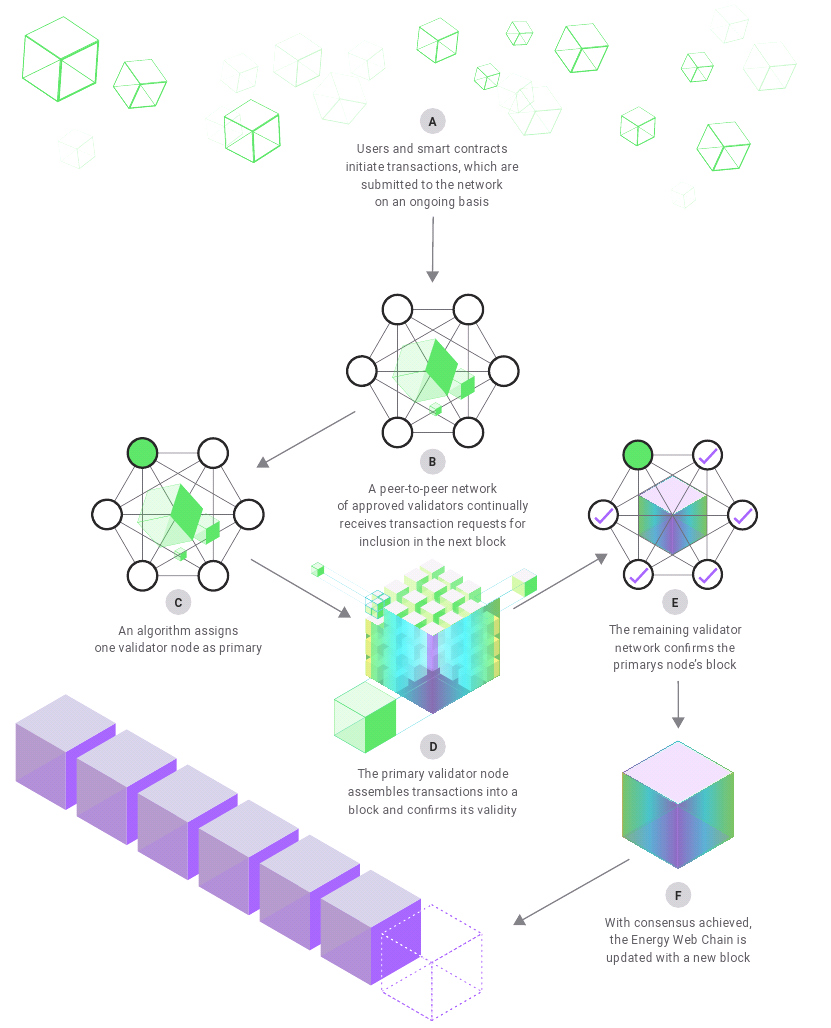
\includegraphics[height=14cm,keepaspectratio]{ew-poa.jpg}
    \centering
    \caption{Passi dell'algoritmo \gls{poa} \cite{img:ew-poa}}
    \label{lab:ew-poa}
\end{figure}


\section{Costi di transazione}
Una transazione è una qualsiasi operazione che modifica lo stato della blockchain. Trasferire token fra account, creare un nuovo smart contract o modificarne lo stato sono esempi di transazioni. \\
Ogni transazione ha un costo che sarà pagato in \gls{ewt}.
Grazie alla specificità di utilizzo della \gls{ewc} e all'algoritmo di consenso, che insieme contribuiscono a ridurre la congestione della rete aumentandone il throughput, 
le tariffe sono generalmente molto basse e vanno da $0.00001$ a $000000.1$ \gls{ewt} \cite{art:manage-costs}. \\
Il costo monetario da pagare per poter effettuare una transazione lo si può calcolare a partire dai seguenti fattori:

\begin{itemize}
    \item \textbf{Il costo in gas:} il gas rappresenta la complessità computazionale necessaria per risolvere la transazione. Più è complessa l'operazione più gas sarà richiesto
    \item \textbf{Prezzo del gas:} valore dell'unità di gas in EWT. Prima di effettuare una transazione, l'utente stabilisce quanto è disposto a pagare per unità di gas. Più è alta l'offerta, maggiore sarà la priorità della transazione
    \item \textbf{Valore di mercato del token:} se si vuole ottenere il costo della transazioni in moneta fiat, basta effettuare la conversione fra EWT spesi e il loro valore monetario
\end{itemize}

Riassumendo con una formula \cite{wiki:ew-transaction-cost}: \\
$ costo(\$) = costo\ gas(gas) * prezzo\ gas(token/gas) * valore\ token (\$/token) $. 


\section{Transazioni private}
Una delle caratteristiche fondanti di ogni blockchain è la possibilità di tracciare e verificare ogni transazione che avviene sulla chain. \\
Questa proprietà fondamentale, però, non è sempre desiderabile: anche per ottemperare alle regolamentazioni vigenti riguardanti la privacy, è necessario che ci sia la possibilità di nascondere informazioni sensibili a soggetti non autorizzati. \\
Sono stati quindi individuati diversi approcci per risolvere il problema.
Di seguito sono elencati i più promettenti e avanzati.
Per una lista completa è possibile consultare la documentazione \cite{wiki:ew-privacy}.

\subsection{Parity Secret Store}
Un'implementazione promettente per risolvere il problema è il Secret Store del client Parity Ethereum. \\
L'idea è quella di generare una coppia di chiavi, pubblica e privata.
Quella pubblica è nota, ed è utilizzata per crittografare i messaggi.
Tuttavia, per decriptare i messaggi, è necessaria la chiave privata.
Questa viene distribuita fra $n$ nodi, in modo che per poter accedere alle informazioni protette sia necessario che un numero arbitrario $m$ su $n$ di questi sia favorevole. \\
La tecnica crittografica utilizzata è la "elliptic curve threshold encryption" \cite{art:ecdkg}. \\
L'implementazione è quella di un \gls{kms}, che invece di essere centralizzato è distribuito.
La decentralizzazione elimina il \gls{spf}, in quanto nessun nodo singolo ha accesso all'intera chiave. \\
Il sistema di consenso può sfruttare un sistema di votazione simile a quello usato per la governance. \\
Vi sono, però, vari limiti all'uso di questa tecnica.
Infatti, è richiesto una setup iniziale fra i nodi interessati, compresa una rete separata per i servizi e le API.
Un numero di nodi attivi deve essere garantito in ogni momento per raggiungere il limite inferiore di votanti.
Infine, attualmente l'implementazione è limitata al client Parity / OpenEthereum.

\subsubsection{Parity Private Transactions}
Continuando a costruire sopra il Parity Secret Store, si può immaginare di generare uno smart contract criptato (\autoref{lab:ew-privacy}).
Questo verrebbe poi inserito dentro uno smart contract tradizionale pubblico sulla blockchain. \\
A quel punto, solo gli account autorizzati, con le chiavi necessarie, sono in grado di leggere e modificare lo stato del contratto interno.
La nuova transazione viene eseguita e firmata off-chain, e il nuovo stato, criptato, viene reinserito nella blockchain pubblica.

\begin{figure}[ht]
    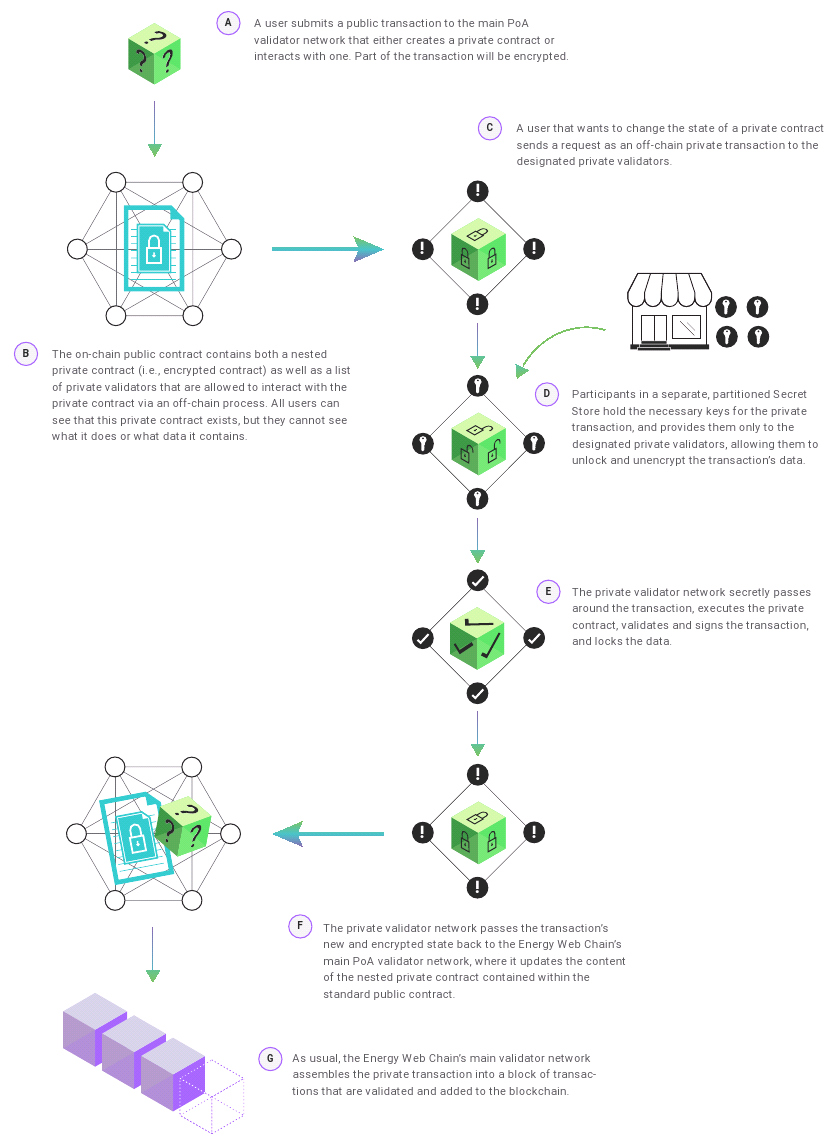
\includegraphics[height=13cm,keepaspectratio]{ew-privacy.jpg}
    \centering
    \caption{Utilizzo di Parity Private Transaction \cite{img:ew-privacy}}
    \label{lab:ew-privacy}
\end{figure}

\subsection{Precise Proofs}
Precise Proofs è uno schema basato sugli alberi di Merkle, in grado di verificare l'autenticità della struttura dati rivelando solo un subset di dati. \\
Si parte realizzando un albero di Merkle a partire dai dati interessati e si rende pubblica la radice. \\
Un terzo ente, interessato a verificare la validità di un subset di dati, riceverà solo i dati effettivamente richiesti e le hash dei dati non necessari.
In questo modo si hanno abbastanza informazioni da poter ricostruire la radice minimizzando i dati resi pubblici.

\subsection{Zero Knowledge Proof Protocols}
Gli Zero Knowledge Proof Protocols sono una categoria di protocolli con lo scopo di validare una computazione senza rivelarne alcun input (es. validare una transazione senza rivelare mittente, destinatario, movimento etc.).

\subsubsection{zkSNARKs}
zkSNARKs è probabilmente il protocollo più avanzato in questa categoria, sviluppato dal team Zcash \cite{wiki:zkSNARKs}.
Sebbene sia il più maturo, presenta un tallone d'Achille non indifferente. \\
Per poter utilizzare la Zero Knowledge Proof è necessario realizzare un circuito aritmetico che rappresenta la computazione da provare e generare da quello una coppia di chiavi prover/verifier.
La creazione di questo setup deve essere sicura e pattuita a priori, perché se dovesse essere compromesso un avversario potrebbe approfittarne per realizzare prove false.


\section{Storage}
Il fatto che tutti i dati siano immagazzinati sulla blockchain per essere accessibili si traduce in un incremento della memoria necessaria per salvare l'intera blockchain su un dispositivo fisico, 
in una maggiore congestione della rete con conseguente calo di prestazione e in un aumento di costi possibilmente evitabili nelle esecuzione degli smart contract. \\
Una prima soluzione è di evitare di immettere dati sulla blockchain, e limitarsi ad utilizzare gli hash degli stessi, per poi limitarsi a verificarne la validità off-chain. \\
Nei casi in cui il salvataggio dei dati fosse necessario, si può provare ad optare per una delle tante soluzioni che offrono un servizio di storage distribuito. \\
Le principali soluzioni sono \gls{ipfs} e Storj.
Per una lista completa è possibile consultare la documentazione \cite{wiki:ew-storage}

\subsubsection{InterPlanetary File System (IPFS)}
\gls{ipfs} \cite{prod:ipfs} è un modello di filesystem distribuito.
Invece di indirizzare i file con la loro locazione, li si identifica con un hash ottenuto dal loro contenuto.
Se il file è troppo grande, lo si spezza in più parti con lo stesso risultato. \\
I nodi che fanno parte di questa rete si auto-iscrivono in delle tabelle di \gls{dht} che tengono traccia dei nodi che possiedono il file associato ad uno specifico hash. \\
Se si vuole contribuire alla rete, una volta scaricato il file lo si tiene in cache, fornendolo ad altri utenti che lo richiedano. \\
Il fatto che un file sia identificato dal suo hash garantisce inoltre l'integrità del dato e la sua immutabilità.
Per aggiornare un file, infatti, bisogna utilizzare il sistema di versioning previsto dal protocollo. \\ \\

\subsubsection{Storj}
Storj \cite{prod:storj} è molto simile ad IPFS, con l'incentivo che i nodi sono pagati per svolgere la loro funzione di content-storage.
Ovviamente il contratto prevede che l'host sia in grado fornire su richiesta in qualsiasi momento tutti i file che afferma di possedere.


\section{Governance}
La natura decentralizzata della blockchain rende un qualsiasi cambiamento che riguarda la sua infrastruttura un problema non banale. \\
Per gestire al meglio i possibili aggiornamenti che la \gls{ewc} potrebbe necessitare, si è deciso di affidarsi a chi la comprende bene, cié gli sviluppatori.
Il diritto di voto che determina quali proposte di modifica vengano accolte e quali respinte sarà determinato dalla quantità di gas che un singolo sviluppatore riesce a "generare" con i propri smart contracts.
L'idea è che il valore che lo sviluppatore fornisce all'intero sistema rappresenta il suo peso nella votazione \cite{wiki:ew-governance}. \\
Ciò non esclude che, in caso si renda necessario, alcune scelte troppo complesse possano essere prese da persone designate senza passare per il meccanismo di voto della blockchain.

\begin{figure}[h]
    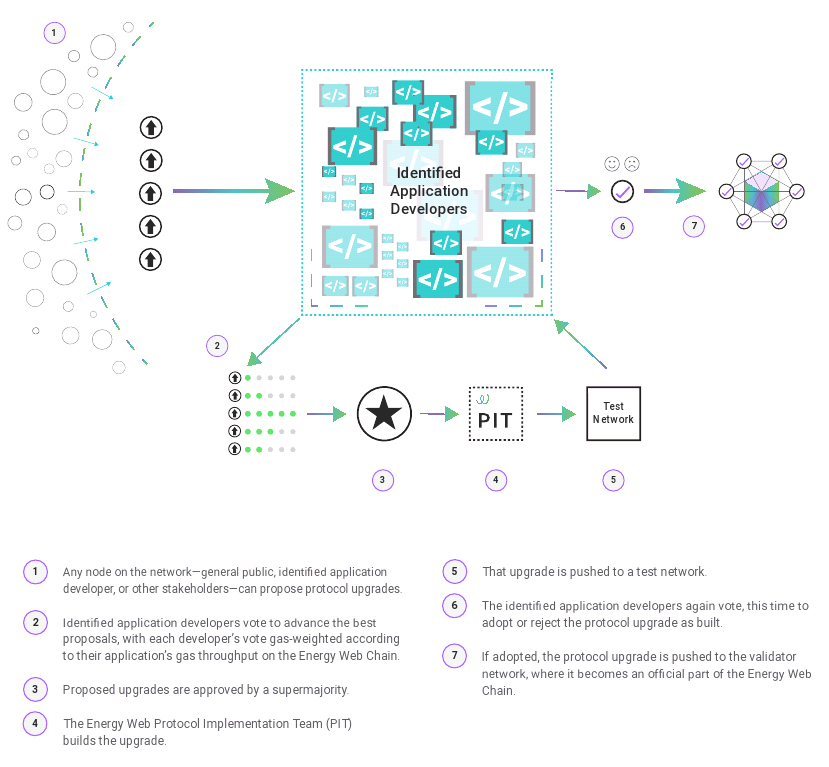
\includegraphics[height=10cm,keepaspectratio]{ew-governance.jpg}
    \centering
    \caption{Passi per l'approvazione di una modifica all'infrastruttura di \gls{ewc} \cite{img:ew-governance}}
    \label{lab:ew-governance}
\end{figure}


\section{Staking}
\label{sec:staking}
Per fornire quello che nell'architettura di ES-DOS è chiamato "Utility layer", è necessario il contributo di operatori che mettano a disposizione le proprie risorse a chi ha intenzione di sviluppare un servizio.
Perché il tutto sia affidabile e adatto ad un ambiente di produzione, devono essere garantiti dei livelli di servizio, in maniera analoga ad un qualsiasi \gls{sla} proposto da un fornitore di SaaS. \\
La soluzione proposta non è dissimile a quella implementata in altre blockchain, e si rifà al modello \gls{pos}.
Gli attori in questo modello vengono suddivisi in due categorie:

\begin{itemize}
    \item \textbf{Service providers:} sono organizzazioni che mettono a disposizione i nodi di utility.
          Per essere approvato, un service provider deve poter dimostrare la propria identità e depositare in garanzia una quantità di EWT per un periodo multi-annale.
          Dopo essere stati approvati, i service providers possono aggiungere ulteriori nodi di utility incrementando proporzionalmente il deposito di EWT.
          Finché lo \gls{sla} continua ad essere rispettato, i service providers guadagneranno un interesse in base al loro deposito.
          In questo momento, il deposito minimo necessario per essere approvati come service provider si attesta fra i $10000$ e i $100000$ EWT, a cui si aggiungono fra i $1000$ e i $10000$ EWT per service node \cite{art:ew-staking}.
    \item \textbf{Patrons:} sono gli individui o le organizzazioni che finanziano un service provider depositando dei loro EWT per il service provider.
          Differentemente rispetto a ciò che accade per i service provider, non c'è un minimo alla somma depositata e questa può essere ritirata in qualsiasi momento.
          Questo porta i patrons a favorire service provider che rispettano gli \gls{sla} e che offrano il miglior modello di revenue-sharing.
\end{itemize}

\begin{figure}[ht]
    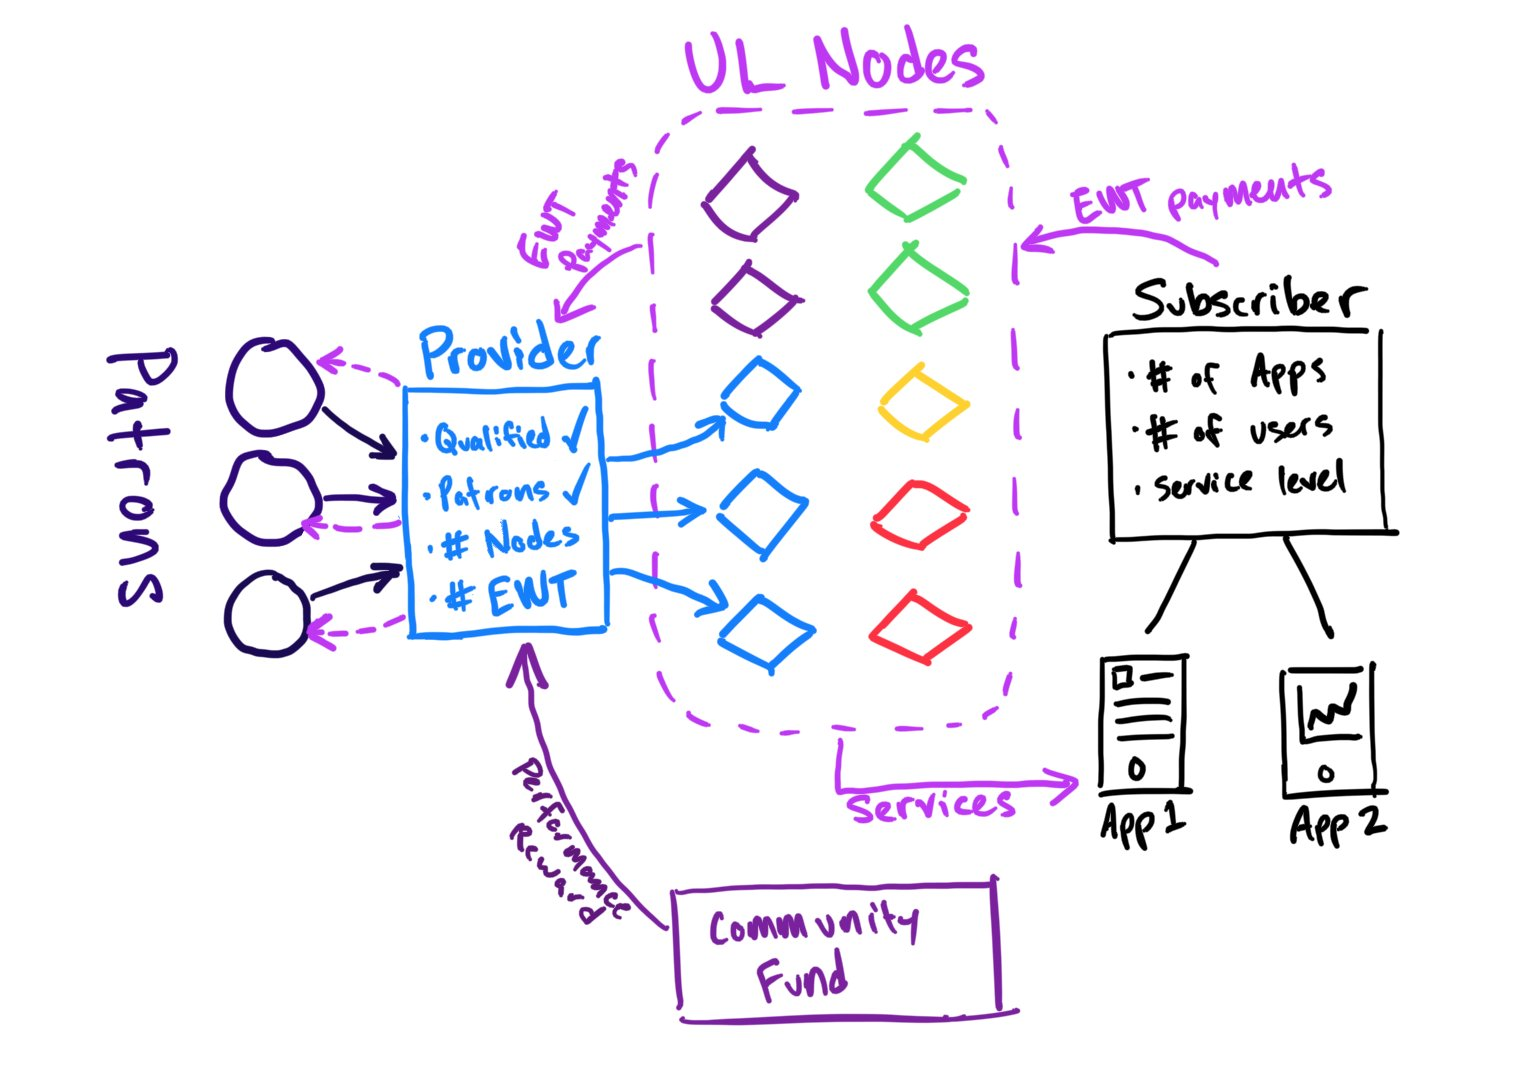
\includegraphics[height=10cm,keepaspectratio]{ew-staking.png}
    \centering
    \caption{Come l'utility layer supportato dallo staking si integra in EW-DOS \cite{art:ew-staking}}
    \label{lab:ew-staking}
\end{figure}

% Energy web services
\chapter{Servizi di Energy Web}

%%%%%%%%%%%%
% Content
%%%%%%%%%%%%
\section{Energy Web Name Service (EWNS)}
\label{sec:ewns}

L'\gls{ens} è un sistema di denominazione distribuito, aperto ed estensibile basato sulla blockchain di Ethereum, ed una sua implementazione è stata resa disponibile anche sulla \gls{ewc}. \\
Analogamente a un DNS, gli indirizzi vengono mappati su nomi di dominio facilmente memorizzabili, dando all'utente un'alternativa all'utilizzo degli indirizzi esadecimali. \\
L'implementazione disponibile pubblicamente consente prevede: indirizzi, indirizzi inversi, hash di dati, definizioni ABI, chiavi pubbliche, interfacce di smart contract e altro \cite{wiki:ewns}.

Per un utente finale il tutto è completamente trasparente. 
È compito dello sviluppatore di DApp integrare le funzionalità dell'ENS. \\
Esistono diverse librerie che già supportano questa funzione, anche se potrebbe essere necessaria qualche patch manuale. \\
Il procedimento per risolvere un dominio con ENS, comunque, non è particolarmente complicato:

\begin{enumerate}
    \item Normalizzare ed applicare una funzione di hashing sul nome \cite{wiki:ens-normalize-name}.
    \item Chiamare la funzione resolver() sul registro ENS, passando l'output del passaggio 1. Ciò restituisce l'indirizzo del resolver responsabile del dominio
    \item Usando l'interfaccia del resolver, chiamare la funzione addr() sull'indirizzo del resolver restituito nel passaggio 2, passando come parametro l'hash trovato nel passaggio 1. In alternativa, se non si sta cercando un indirizzo, chiamare la funzione dell'interfaccia prevista, ad esempio text()
\end{enumerate}

\section{Decentralized IDentifiers (DIDs)}
\label{sec:did}

I \gls{did} sono identificatori univoci usati per realizzare identità digitali verificabili e decentralizzate. Sono la base per l'implementazione delle \gls{ssi} \cite{art:ssi}. \\
Il soggetto identificato può essere qualsiasi cosa: una persona, un'organizzazione o un bene fisico, per fare qualche esempio. \\
Un \gls{did} si comporta come un URI e punta ad un DID document, archiviato su un archivio pubblico permanente, come una blockchain.
Questo documento contiene tutte le caratteristiche (claims), ad esempio certificazioni o autorizzazioni, che si riferiscono al corrispettivo \gls{did}. \\
Chiunque può creare un nuovo \gls{did} in qualsiasi momento.

\begin{figure}[ht]
    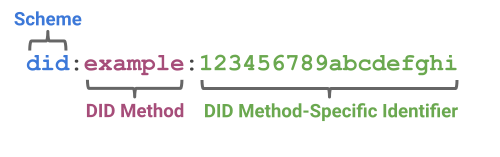
\includegraphics[width=13cm,keepaspectratio]{did-schema.png}
    \centering
    \caption{Composizione di un \gls{did} \cite{img:did-schema}}
    \label{lab:did-schema}
\end{figure}

Un \gls{did} è una stringa composta da tre parti (\autoref{lab:did-schema}): lo schema did:, un metodo e un identificatore univoco rispetto al metodo \cite{wiki:did}. \\
I documenti \gls{did}, invece, sono dei file JSON-LD \cite{wiki:json-ld}. Il documento \gls{did} contiene tutte le informazioni, o claims, 
relative al soggetto identificato dal \gls{did} e fornisce una serie di meccanismi che consentono a un controller del \gls{did} di dimostrare il proprio controllo sul \gls{did}. 
Tipicamente esprimono anche metodi di verifica, come chiavi pubbliche crittografiche, e servizi relativi alle interazioni con il soggetto \gls{did}. \\
Il controller di un \gls{did} è l'entità che ha la capacità di apportare modifiche a un documento \gls{did}. Questa capacità in genere è subordinata dal possesso dal possesso della coppia di chiavi crittografiche. 
Si noti che un \gls{did} potrebbe avere più di un controller e il soggetto \gls{did} può essere il controller \gls{did} o uno di essi. \\
I sistemi che supportano la registrazione dei \gls{did} e la restituzione dei dati necessari per produrre documenti \gls{did} sono chiamati "verifiable data registry". \\
Un risolutore \gls{did} è il componente che, dato un \gls{did}, restituisce il documento corrispondente. Questo processo è chiamato risoluzione \gls{did} (\autoref{lab:did-architecture}).

\begin{figure}[ht]
    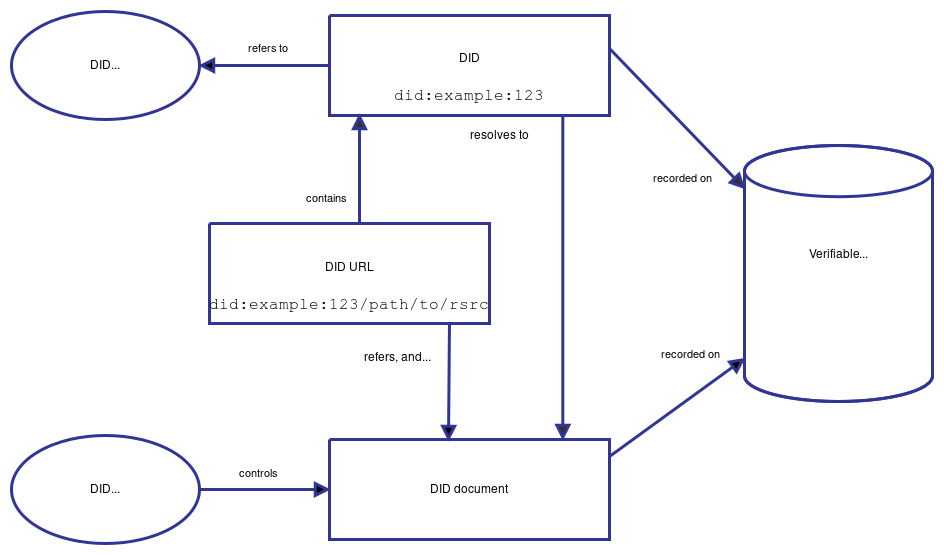
\includegraphics[width=13cm,keepaspectratio]{did-architecture.png}
    \centering
    \caption{Panoramica dell'architettura dei \gls{did} e le relazioni fra le componenti fondamentali \cite{img:did-architecture}}
    \label{lab:did-architecture}
\end{figure}

Il soggetto identificato ha bisogno di un’identità per essere in grado di dimostrare di possedere determinati tratti o caratteristiche a un verificatore. \\
Il verificatore ha un certo numero di emittenti di fiducia ed è disposto ad accettarne i claims, cioè le affermazioni.
Il soggetto può chiedere a uno di questi emittenti di aggiungere una dichiarazione firmata sul proprio documento \gls{did}. 
Inoltre, sia l'emittente che il verificatore devono essere in grado di verificare che il soggetto sia effettivamente il proprietario dell'identità. 
Ciò si ottiene tramite DIDAuth. \\
Questo processo può assumere molte forme, come specificato nel documento \gls{did}, ma un modo comune è attraverso un challenge inviata dall'emittente o dal verificatore al soggetto, 
del quale conoscono la chiave pubblica grazie al DID document, che a sua volta risponderà firmando con la propria chiave privata, dimostrando la propria identità.

\subsubsection {Analogia con il mondo reale} 
Si vuole comprare alcool al bar. Per farlo, si deve essere in grado di dimostrare al barista di avere almeno 18 anni. Il barista in questo caso è il verificatore.
Si può dimostrare la richiesta mostrando la propria carta d'identità.
Questa viene rilasciato dal governo, che funge da emittente di fiducia per il barman, 
il quale verificherà che il richiedente sia effettivamente la persona raffigurata nella foto e si convincerà che del possesso del requisito della maggiore età.

\begin{figure}[ht]
    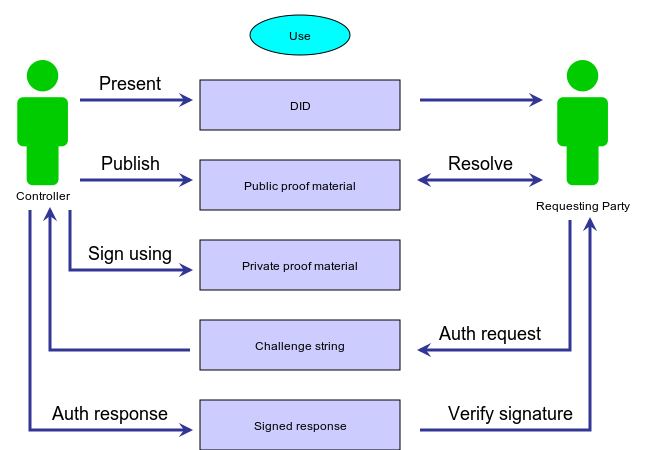
\includegraphics[width=13cm,keepaspectratio]{did-auth.png}
    \centering
    \caption{Panoramica dell'architettura dei \gls{did} e le relazioni fra le componenti fondamentali \cite{img:did-auth}}
    \label{lab:did-auth}
\end{figure}

Le blockchain, grazie alle loro caratteristiche, si sono rivelate un sistema ideale per integrare un sistema di \gls{ssi}, anche in ambiti che esulano il settore energetico \cite{art:blockchain-did}. \\
Nel progetto di \gls{ew} i \gls{did} ricoprono un ruolo centrale. 
Ogni utente può richiedere un \gls{did} che mantenga la lista di claims verificabili che l'utente possiede.
È anche possibile assegnare un \gls{did} ad ogni \gls{der}, così da tenere traccia di tutte le informazioni e certificazioni legate a quello specifico \gls{der}. \\

Altri vantaggi forniti da questo sistema sono:
\begin{itemize}
    \item Meccanismo di autenticazione - Il soggetto è in grado di fornire una prova crittografica del proprio controllo sul \gls{did}
    \item Autorizzazione e deleghe -  Il protocollo prevede la possibilità per un \gls{did} di autorizzare o delegare un altro \gls{did} per permettergli di effettuare operazioni a suo nome
\end{itemize}

\section{Identity and Access Management (IAM)}
\label{sec:iam}

\gls{iam} è un insieme di policy in grado di garantire che solo le entità con le credenziali e le autorizzazioni necessarie possano accedere alle risorse. \\
Il sistema deve prima controllare l'identità digitale del soggetto e verificare i ruoli ad esso associati.
L'operazione viene autorizzata solo se il soggetto ha i ruoli necessari.
Per assicurare l'\textit{accountability}, viene utilizzato un sistema di \textit{logging} per registrare ogni operazione eseguita dal soggetto.\\

Per implementare un sistema IAM decentralizzato bisogna garantire alcune proprietà. 

\textbf{L'IAM deve essere resistente alla censura.}
Significa che non esiste alcun attore nel sistema che abbia il potere di limitare selettivamente le informazioni a cui gli altri hanno accesso.
Questo aspetto è importante perché informazioni riguardanti situazioni casi in cui un'autorizzazione o una chiave è stata revocata o invalidata o se è stata appena concessa un'autorizzazione devono essere disponibili pubblicamente. \\
Una blockchain, per sua natura, soddisfa questi requisiti. Inoltre, le prove crittografiche contenute nelle transazioni consentono la verifica off-line dei dati.
Le descrizioni dei ruoli sono contenute in uno smart contract ENS, mentre l'avvenuta concessione di un ruolo e i suoi dettagli è annotata nel documento DID dell'utente, mantenuto off-chain.

\textbf{Le informazioni su utenti e ruoli devono essere riservate.}
Nella soluzione di Energy Web, nessuna terza parte dispone dell'elenco completo degli utenti di un'applicazione. \\
Ciò è garantito dal processo di concessione dell'autorizzazione, poiché è l'utente che archivia il claim e ne aggiunge la descrizione sulla blockchain, consentendogli di dimostrare che gli è stato concessa una determinata autorizzazione (\autoref{lab:iam-process}). \\
Poiché si tratta di una operazione svolta dall'utente stesso, i contenuti del ruolo non sono divulgati \cite{img:iam}.
L'unica informazione che un osservatore può raccogliere è che l'utente ha aggiunto un claim al proprio DID document, ma non il contenuto, l'origine o la natura del claim. \\

\begin{figure}[ht]
    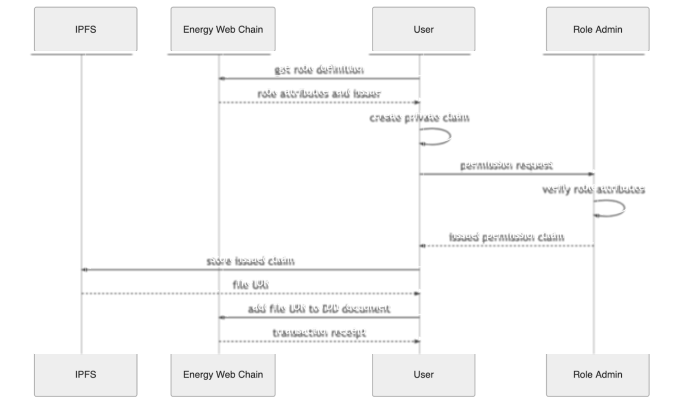
\includegraphics[width=13cm,keepaspectratio]{iam-process.png}
    \centering
    \caption{Processo di rilascio dei ruoli \gls{iam} \cite{img:iam}}
    \label{lab:iam-process}
\end{figure}

Anche l'\gls{iam} rappresenta un punto cardine nel progetto \gls{ew}. \\
Attraverso il suo utilizzo, è possibile creare delle organizzazioni con una struttura gerarchica, simile ai domini attualmente utilizzati sul web.
I ruoli che gli utenti possiedono determinano le azioni che possono compiere all'interno dell'organizzazione. \\
La gestione di tutti questi aspetti è stata resa molto più accessibile grazie alla \gls{dapp} \href{https://switchboard.energyweb.org/}{Switchboard} (\url{https://switchboard.energyweb.org/}).

% Conclusion
\chapter*{Conclusione}
\addcontentsline{toc}{chapter}{Conclusione} % add the chapter to the index
È ragionevole assumere che la decentralizzazione della rete elettrica sia un processo inevitabile che coinvolgerà un numero sempre crescente di utenze, 
sia nel ruolo di consumatori che nel ruolo di produttori. \\

Fra le possibili soluzioni, quella di usare la blockchain come infrastruttura in grado di supportare questo mercato sempre più decentralizzato sembra essere particolarmente promettente. \\
Ad una analisi approfondita \gls{ew} risulta essere un progetto con una visione ed un focus chiari, guidato da persone che hanno le conoscenze necessarie per creare una piattaforma ad hoc per questo settore. \\
Proprio in virtù di ciò, le tecnologie che \gls{ew} impiega non sono necessariamente innovative.
Si cerca, al contrario, di seguire ed implementare quanti più standard possibile, e partire da questi per fornire dei servizi che rendano appetibile l'intera infrastruttura. \\
La scelta di rendere tutto il materiale, le implementazioni e le librerie open-source è in linea con la volontà di fornire degli strumenti che facilitino la vita agli sviluppatori, 
sui quali poi ricade il compito di creare \gls{dapp} e servizi per l'utente finale. \\
È bene, infine, tenere a mente che \gls{ew}, al momento della stesura di questo documento, è un progetto in divenire, e, per questo, soggetto a continui cambiamenti.
Nonostante ciò, penso che \gls{ew} fornisca quantomeno un ottimo caso di studio che valga la pena approfondire per chi fosse interessato ad affrontare la problematiche trattate nell'introduzione del documento.


% Energy Web showcase
\chapter*{Progetto}
\addcontentsline{toc}{chapter}{Progetto} % add the chapter to the index
Ad affiancare questa relazione è stata realizzata una demo implementativa che è possibile provare navigando all'indirizzo \url{https://tendto.github.io/EW-showcase/}.
Al fine di visionare tutte le funzioni, è necessario dotarsi dell'estensione browser \href{https://metamask.io/}{MetaMask}, \href{https://energyweb.atlassian.net/wiki/spaces/EWF/pages/703201459/Volta+Connecting+to+Remote+RPC+and+Metamask}{connettersi alla rete Volta} e avere a disposizione qualche \href{https://voltafaucet.energyweb.org/}{Volta token}. \\

La \gls{dapp} (\autoref{lab:project}) rappresenta la sintesi del progetto, e ha come scopo quello di mostrare in azione le funzionalità \gls{ewns} (\autoref{sec:ewns}), \gls{did} (\autoref{sec:did}) e \gls{iam} (\autoref{sec:iam}), utilizzando, ove possibile, le librerie e i frameworks messi a disposizione da \gls{ew}.

\begin{figure}[h]
    \centering
    \subfloat[\centering \gls{did}]{{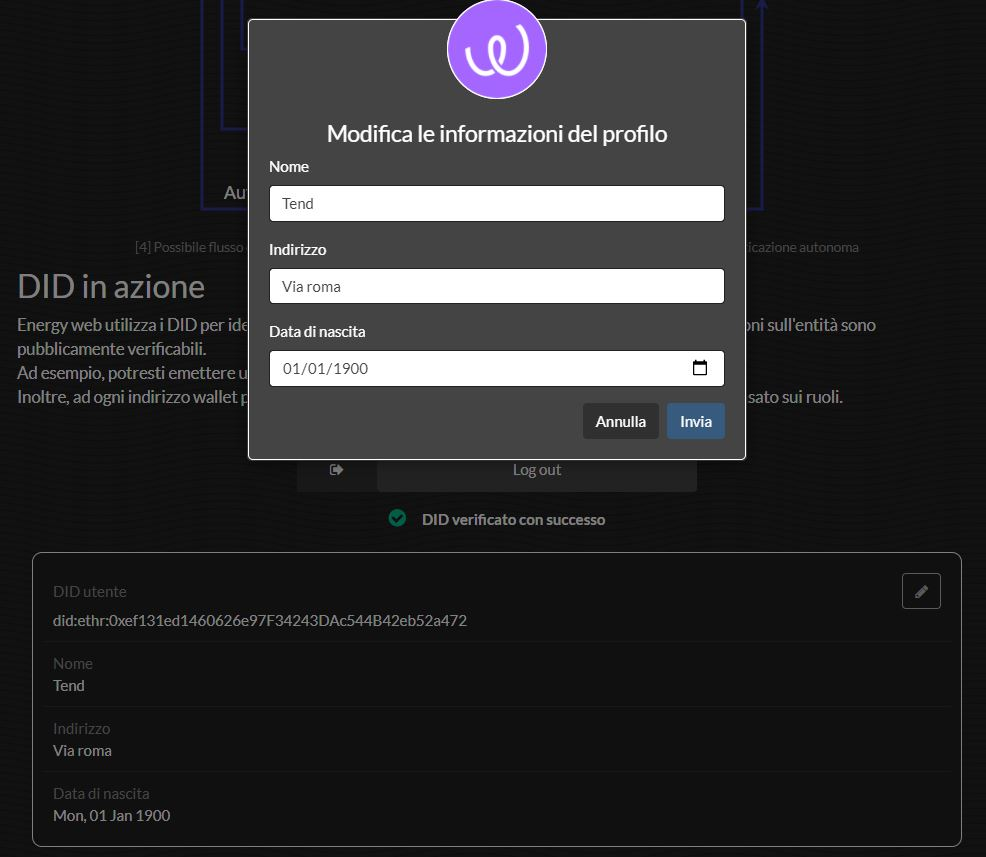
\includegraphics[width=6cm]{DID.jpg} }}
    \qquad
    \subfloat[\centering \gls{iam}]{{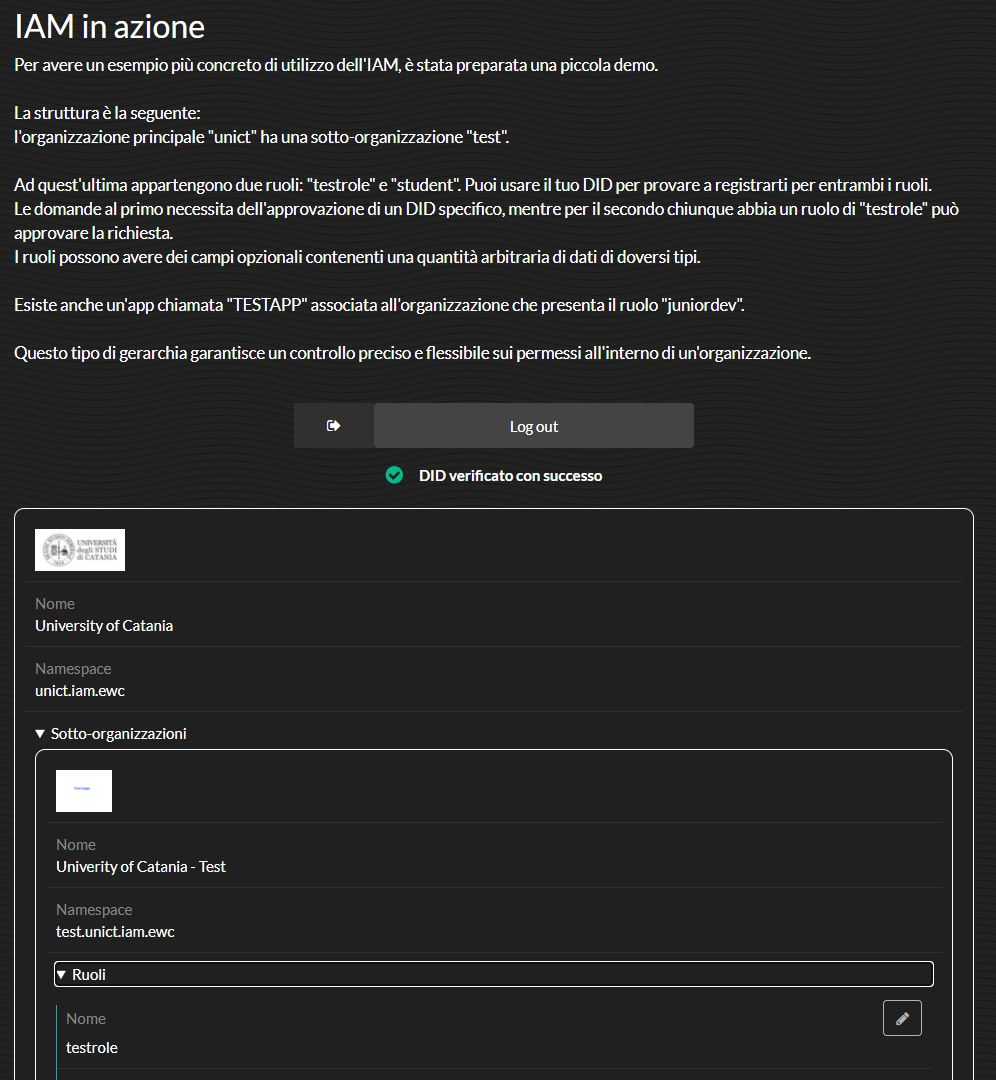
\includegraphics[width=6cm]{IAM.jpg} }}
    \caption{Screenshots della \gls{dapp}}
    \label{lab:project}
\end{figure}

\begin{figure}[h]
    \centering
    \subfloat[\centering Proprietario]{{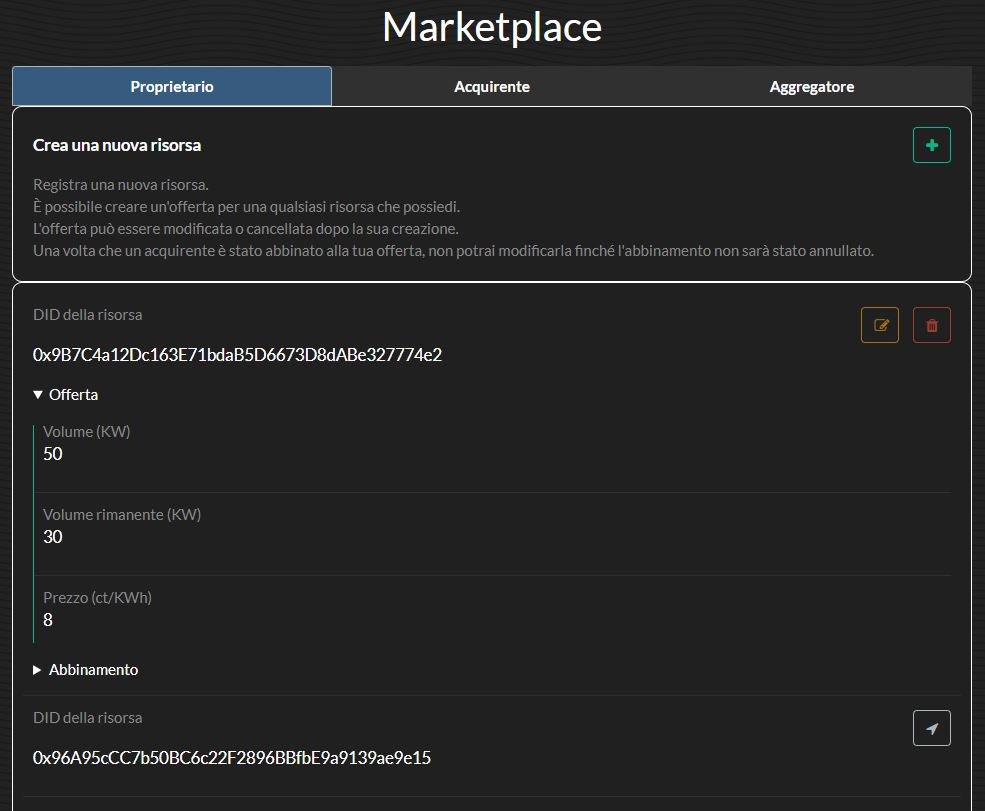
\includegraphics[width=6cm]{Marketplace1.jpg} }}
    \qquad
    \subfloat[\centering Aggregatore]{{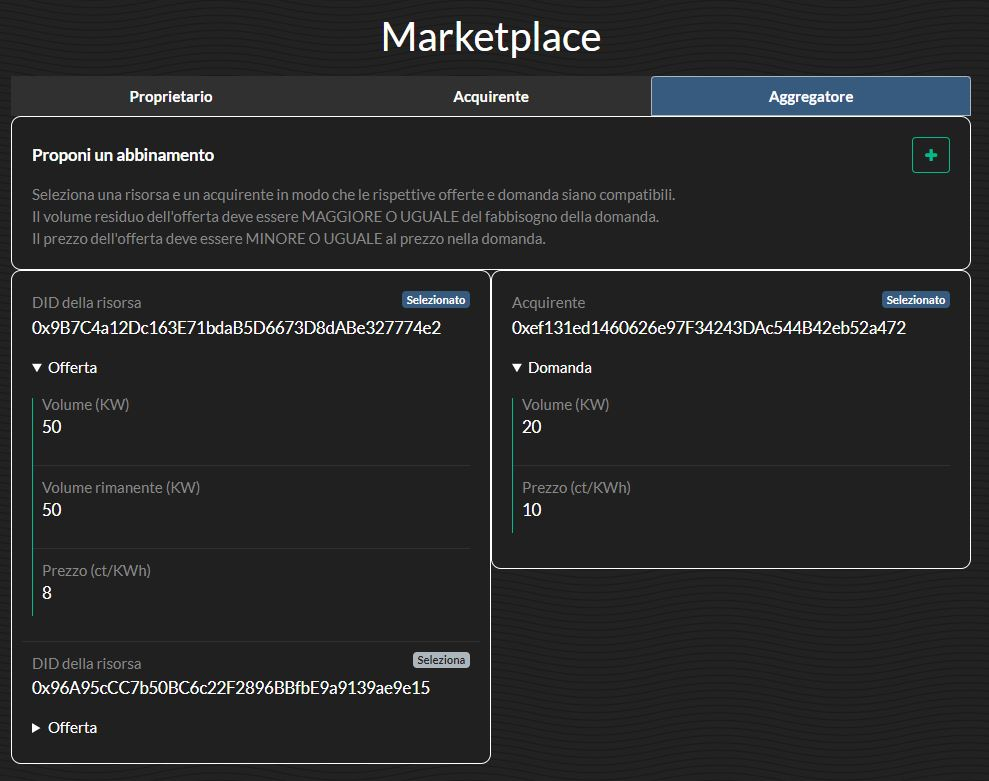
\includegraphics[width=6cm]{Marketplace2.jpg} }}
    \caption{Screenshots del Marketplace}
    \label{lab:marketplace}
\end{figure}

L'ultima sezione della \gls{dapp} comprende una implementazione molto semplificata di Energy Web Flex, chiamata Marketplace (\autoref{lab:marketplace}). \\

\newpage
Vengono individuati tre ruoli chiave: 
\begin{itemize}
    \item il proprietario di \gls{der} (\textbf{P}) - vende energia
    \item l'acquirente (\textbf{A}) - acquista energia
    \item l'aggregatore (\textbf{AGG}) - abbina domanda e offerta
\end{itemize}

Creare un abbinamento fra il primo e il secondo richiede generalmente il seguente procedimento:
\begin{enumerate}
    \item \textbf{P} propone un'offerta per i \gls{der} che possiede, specificando il volume di energia (kW) e il prezzo (ct/kWh). L'offerta può essere modificata o ritirata successivamente
    \item \textbf{A} pubblica una domanda con il volume di energia (kW) di cui ha bisogno e il prezzo massimo (ct/KWh) che è disposto a pagare. La domanda può essere modificata o ritirata successivamente
    \item AGG seleziona un'offerta e una domanda che formino una coppia valida e propone l'abbinamento. Da questo momento in poi offerta e domanda non possono più essere modificate fino a quando l'abbinamento proposto non viene accettato o rifiutato
    \item L'abbinamento proposto può essere accettato solo da \textbf{A}, ma può essere rifiutato sia da \textbf{P} che da \textbf{A}
    \item Una volta accettato, l'abbinamento entra in vigore.
    \item In qualsiasi momento sia \textbf{P} che \textbf{A} possono eliminare l'abbinamento
\end{enumerate}

Il Marketplace utilizza due smart contract presenti sulla Volta testnet:
\begin{itemize}
    \item \href{https://volta-explorer.energyweb.org/address/0x84d0c7284A869213CB047595d34d6044d9a7E14A/transactions}{Identity Manager (0x84d0c7284A869213CB047595d34d6044d9a7E14A)}, smart contract ufficiale sviluppato ed utilizzato da \gls{ew}
    \item \href{https://volta-explorer.energyweb.org/address/0x37dfeF9b9c56A81927Dfa73994E2fb23c3dd4b37/transactions}{Marketplace (0x37dfeF9b9c56A81927Dfa73994E2fb23c3dd4b37)}
\end{itemize}

L'intera documentazione e il codice dell'implementazione sono disponibili nella repository pubblica \href{https://github.com/TendTo/EW-showcase}{EW showcase} (\url{https://github.com/TendTo/EW-showcase}) su Github.

% Glossaries and bibliografy
\printnoidxglossary
\printbibliography[heading=bibintoc]

\end{document}